\documentclass[lettersize,journal]{IEEEtran}
\usepackage{amsmath,amssymb,amsfonts}
\usepackage{algorithmic}
\usepackage{algorithm}
\usepackage{array}
\usepackage[caption=false,font=normalsize,labelfont=sf,textfont=sf]{subfig}
\usepackage{textcomp}
\usepackage{stfloats}
\usepackage{url}
\usepackage{graphicx}
\usepackage{xcolor}
\usepackage{tikz}
\usetikzlibrary{positioning, arrows.meta, shapes.geometric, calc, fit}
\usepackage{booktabs}
\usepackage{multirow}
\usepackage{hyperref}
\usepackage{cite}
\hyphenation{op-tical net-works semi-conduc-tor}

\begin{document}

\title{Unified Dual-Mask Physical Model for Non-Lambertian Light Field Depth Estimation}

\author{Ruifeng Huang and Zhenglong Cui
\thanks{Manuscript received May 2026. This work was supported by Beihang University. (Corresponding author: Zhenglong Cui)}
\thanks{R. Huang and Z. Cui are with the School of Computer Science and Engineering, Beihang University, Beijing, China (e-mail: huangruifeng@buaa.edu.cn; czl@buaa.edu.cn).}}

\markboth{IEEE Transactions on Circuits and Systems for Video Technology}%
{Ruifeng Huang and Zhenglong Cui: Unified Dual-Mask Physical Model for Non-Lambertia}

\maketitle

\begin{abstract}
Light field depth estimation is substantially challenged by non-Lambertian reflections, which violate the angular consistency assumption inherent in epipolar plane image (EPI) analysis. Existing EPI-based and purely data-driven methods suffer from severe degradation in specular and scattering regions, often degenerating into texture replication due to a lack of physical interpretability. To address this limitation, a Unified Dual-Mask Physical Model was developed to integrate signal-processing rigor with physical optics. Specifically, a k-space-inspired angular frequency analysis was introduced that applied 2D discrete Fourier transforms to the angular sampling matrix to decouple low-frequency diffuse and high-frequency specular components. Furthermore, a dual-mask physical modeling module generated a media mask for material weighting and an angular mask for wavevector deflection, constraining bidirectional reflectance distribution function parameters via radiation tensor field rank assumptions. Finally, a component-aware adaptive fusion strategy independently processed diffuse, specular, and scattering depth components, integrating them via confidence-weighted optimization. Extensive evaluations across three datasets demonstrate that the proposed method reduces the mean absolute error (MAE) in non-Lambertian regions by 43.1% (achieving 0.234) compared to the EPI baseline, while maintaining an overall mixed-scene MAE of 0.181 with only 108K parameters. This work establishes a physically interpretable and computationally efficient paradigm for complex light field image processing.
\end{abstract}

\begin{IEEEkeywords}

\end{IEEEkeywords}

\section{1. Introduction}

Light field (LF) imaging has revolutionized 3D computer vision by simultaneously capturing both the spatial and angular distribution of light rays \cite{lightfieldimaging3Dreconst}. This rich multidimensional representation implicitly captures the 3D geometry and material properties of a scene, making LF depth estimation a cornerstone for downstream applications such as autonomous navigation, robotic manipulation, and immersive virtual reality \cite{autonomousnavigationrobotic}. Conventionally, the majority of LF depth estimation algorithms heavily rely on the Epipolar Plane Image (EPI) and the fundamental assumption of photo-consistency, which posits that the radiance of a Lambertian surface point remains constant across different viewpoints \cite{EpipolarPlaneImagesphotoco}. Under this ideal Lambertian assumption, existing learning-based and geometry-based frameworks have achieved remarkable success, yielding highly accurate depth maps in controlled environments.

However, obtaining the precise shape of glossy, specular, or translucent objects—ubiquitous in our daily lives as metals, plastics, and ceramics—remains a formidable challenge, since standard Lambertian cues like photo-consistency cannot be easily applied \cite{glossyobjectsspecularreflec}. Real-world LF images frequently encounter spatially-varying BRDFs (SVBRDFs) and complex reflections. This difficulty arises because Non-Lambertian surfaces introduce misleading visual information about scene geometry; for instance, specular highlights shift non-linearly with viewpoint changes, while subsurface scattering blurs the angular correspondence \cite{spatiallyvaryingBRDFsmislea}. Such situations substantially break the Lambertian assumptions, leading to the catastrophic failure of most existing depth estimation algorithms that solely depend on angular photo-consistency \cite{Lambertianassumptionsangular}. Furthermore, inferring the depth of these complex surfaces represents a hard challenge not only for conventional geometric algorithms but also for modern deep neural networks, which often struggle to disentangle the intertwined effects of geometry and reflectance from limited angular samples \cite{deepneuralnetworksdisentang}.

The severity of this performance degradation is starkly evident in empirical evaluations. For example, representative EPI-based baselines, such as EPINet variants, demonstrate exceptional proficiency in mixed or predominantly Lambertian domains, achieving a Mean Absolute Error (MAE) as low as 0.081. In stark contrast, when evaluated on purely Non-Lambertian subsets, their performance dramatically deteriorates, with the MAE surging to over 0.411. More critically, visual inspections reveal that in Non-Lambertian regions, the network's predictions completely degenerate into a mere replication of the input RGB textures (i.e., "texture copying") rather than recovering the underlying depth structures. This phenomenon indicates that the model has entirely abandoned geometric reasoning in the absence of valid photo-consistency cues. Additionally, the problem is exacerbated by severe data scarcity and imbalance; high-quality Non-Lambertian LF datasets are exceptionally rare  [e.g., merely 4 training scenes compared to 170 mixed scenes in standard benchmarks], causing data-driven models to severely overfit to Lambertian priors. Even in purely Lambertian scenes, complex textures often cause EPI slope blurring, creating a performance plateau  [e.g., MAE stagnating around 0.32-0.38] that cannot be breached by mere hyperparameter tuning or network scaling.

Therefore, addressing the depth estimation of Non-Lambertian and mixed scenes is not merely an incremental improvement, but an urgent necessity for deploying LF technologies in unconstrained real-world environments. On the one hand, the definition of depth itself might appear ambiguous in the presence of transparent or mirror (ToM) layers; on the other hand, as humans can effortlessly perceive 3D structures through experience and subtle visual cues, depth sensing techniques based on explicit physical modeling hold the potential to address this under-constrained problem \cite{transparentormirrorsurfaces}. There is a pressing need to shift from purely data-driven, black-box paradigms to physically interpretable models that can explicitly parse material reflection types  [i.e., diffuse, specular, and scattering] from the limited angular samples (e.g., $9 \times 9$ views). By formulating a unified physical model that adaptively decouples and processes different reflection components, we can substantially resolve the fatal flaws of traditional EPI methods and dramatically boost the robustness and accuracy of LF depth estimation across diverse and complex real-world scenarios.

To address the depth estimation of Non-Lambertian surfaces, extensive research has been conducted, which can be broadly categorized into traditional geometry-based methods, early deep learning-based approaches, and recent advanced frameworks. Despite their respective merits, these methods exhibit inherent limitations when confronting spatially-varying BRDFs (SVBRDFs) and complex mixed scenes, primarily due to the violation of the photo-consistency assumption.

Traditional geometry and photometric methods predominantly rely on Epipolar Plane Images (EPIs) and defocus cues to infer depth \cite{traditionalEPImethodsdefocu}. Under the ideal Lambertian assumption, a scene point projects onto a straight line in the EPI, whose slope is inversely proportional to its depth. However, these methods exhibit critical flaws in Non-Lambertian regions. This difficulty arises because specular highlights shift non-linearly across viewpoints, causing EPI lines to break or curve, which leads to the catastrophic failure of slope-based depth estimation, often degenerating into mere texture copying \cite{EPIfailuretexturecopying}. Furthermore, to handle glossy or translucent objects, some traditional approaches introduce polarized filters, active illumination, or rely on restrictive physical priors such as known distant light sources \cite{polarizedfiltersknownlight}. These methods lack a unified physical formulation for mixed scenes, making them highly intrusive and poorly generalizable to unconstrained real-world environments.

With the advent of deep learning, early learning-based methods formulated depth estimation as a regression problem by extracting features from EPIs or constructing cost volumes \cite{EPINetcostvolume}. While these data-driven models significantly improved accuracy in Lambertian scenes, they struggle with Non-Lambertian surfaces primarily due to their black-box nature and lack of physical interpretability \cite{lackofphysicalinterpretabil}. Since the training datasets are mostly composed of Lambertian scenes, these networks implicitly memorize photo-consistency and fail to generalize to specular or scattering regions. To mitigate this, some attempts have been made to increase network complexity, incorporate additional branches (e.g., defocus branches), or utilize higher angular resolutions  [e.g., expanding from $5 \times 5$ to $9 \times 9$ views] \cite{MaterialDualCueNethigherangu}. Nevertheless, empirical evidence suggests that simply adding a defocus branch or increasing the number of views does not necessarily help the network learn effective depth features for Non-Lambertian materials, but rather dramatically increases the computational burden without addressing the underlying physical ambiguities.

More recently, advanced methods have attempted to decouple geometry and reflectance by introducing attention mechanisms, vision transformers, or material-aware modules \cite{attentionmechanismsmaterial}. Although these approaches represent a step forward, they still suffer from two critical bottlenecks. On the one hand, material classification or reflection decoupling typically relies on heavy learning-based classifiers, which struggle to accurately distinguish complex reflection types  [e.g., distinguishing subsurface scattering from specular reflection] from limited angular samples (e.g., $9 \times 9$ views), resulting in high computational complexity and poor real-time performance \cite{heavylearningbasedclassifie}. On the other hand, in the depth fusion stage, these methods generally employ simple masking or global weighting strategies, failing to exploit the physical essence of the Radiance Tensor Field (RTF). Without physically constraining the BRDF parameters based on the rank properties of the RTF, the misleading gradients from Non-Lambertian regions inevitably interfere with the overall optimization, leading to sub-optimal depth maps in mixed scenes \cite{misleadinggradientssuboptim}.

In summary, existing methods either lack a lightweight and physically explicit material prior, or fail to establish a unified physical model and component-aware adaptive fusion strategy for diverse reflection types. Therefore, there is an urgent need for a unified, physically-grounded framework that can explicitly parse material reflection types from limited angular samples, model the light-matter interaction via dual-mask physical modeling, and adaptively fuse depth estimations across decoupled reflection components.

To overcome the inherent limitations of black-box data-driven models and the catastrophic failure of geometry-based methods under the violation of the photo-consistency assumption, we propose a Unified Dual-Mask Physical Model for Non-Lambertian Light Field (LF) depth estimation. In this paper, we explicitly formulate depth inference as a physically grounded, component-aware decoupling and aggregation process. Instead of treating LF depth estimation as a purely empirical regression problem, our framework leverages the intrinsic physical properties of light transport. Specifically, we introduce an MRI-inspired angular frequency analysis to parse material reflection types, construct a dual-mask physical model to unify the representation of Lambertian, Non-Lambertian, and mixed scenes, and design a component-aware adaptive fusion strategy to robustly estimate depth across spatially-varying BRDFs (SVBRDFs).

\begin{itemize}\item \textbf{Contribution 1: MRI-Inspired Angular Frequency Analysis for Material Reflection Parsing.} We propose a novel angular frequency analysis module that draws an analogy between the $9 \times 9$ angular samples of an LF pixel and the k-space frequency domain in Magnetic Resonance Imaging (MRI). By applying a 2D Discrete Fourier Transform (2D-DFT) to the angular sampling matrix, we explicitly decouple the reflection components based on their spectral energy distributions: low-frequency dominance for diffuse reflection, high-frequency broadening for specular reflection, and mid-frequency concentration for scattering. This approach solves the bottleneck of distinguishing complex reflection types from limited angular samples, providing a physically meaningful, lightweight ($\mathcal{O}(HW)$ complexity), and real-time pixel-level tri-classification of material types, which lays a reliable prior foundation for subsequent depth estimation.\end{itemize}

\begin{itemize}\item \textbf{Contribution 2: Dual-Mask Physical Modeling for Unified Scene Representation.} We formulate a Dual-Mask Physical Model comprising a Media Mask and an Angular Mask to explicitly model light-matter interactions. The Media Mask quantifies pixel-level surface roughness to determine the interaction type  [specular, scattering, or diffuse], while the Angular Mask records the deflection vector field to characterize the directional changes of the light wave vector during reflection. Grounded on the physical assumption of the Radiance Tensor Field (RTF) rank  [rank $1$ for Lambertian and $\ge 2$ for Non-Lambertian scenes], we estimate BRDF parameters via constrained least squares fitting of $81$ angular equations. This contribution substantially addresses the lack of physical interpretability in conventional data-driven models, unifying the mathematical modeling of Lambertian, Non-Lambertian, and mixed scenes, and enabling the network to adaptively handle mixed materials and complex illumination conditions.\end{itemize}

\begin{itemize}\item \textbf{Contribution 3: Component-Aware Adaptive Depth Estimation and Fusion Strategy.} We introduce a component-aware fusion strategy that decouples the depth estimation task into diffuse, specular, and scattering components based on the weights derived from the dual-mask model. Specifically, we design tailored depth estimation strategies for each reflection type: employing Epipolar Plane Image (EPI) methods for diffuse regions, attenuating EPI confidence and utilizing photometric stereo or neighborhood propagation for specular regions, and applying scattering model corrections for scattering regions. Furthermore, we incorporate a pixel-level confidence weighting mechanism based on the Media Mask into the loss function to suppress gradient interference from Non-Lambertian regions. This strategy substantially resolves the fatal flaw of traditional EPI methods—which completely fail and degenerate into texture copying in Non-Lambertian regions due to the violation of the photo-consistency assumption—significantly boosting depth estimation accuracy and robustness in mixed and Non-Lambertian scenes.\end{itemize}

Extensive experiments on multiple benchmark datasets  [including HCInew, Non-lambertian, and UrbanLF-Syn] demonstrate that our proposed method significantly outperforms state-of-the-art approaches. Specifically, our model achieves an overall Mean Absolute Error (MAE) of less than $0.20$ on mixed datasets, with MAEs strictly bounded below $0.16$, $0.25$, and $0.22$ on Lambertian, Non-Lambertian, and mixed subsets, respectively. Notably, with an extremely compact parameter size of merely $\sim 108$K, our physically grounded framework exhibits remarkable generalization capability and computational efficiency, validating the effectiveness of integrating explicit physical priors into LF depth estimation.


\section{2. Related Work}

\subsection{Traditional Light Field Depth Estimation Methods}

Many depth estimation methods for light-field cameras have been proposed \cite{lightfielddepthestimationE}. Among the earliest and most influential approaches, Wanner et al. \cite{Wannergloballyconsistentdep} proposed a variational framework that derives depth from the slope of linear structures in Epipolar Plane Images (EPI). By formulating depth estimation as an energy minimization problem, they explicitly enforce photo-consistency across angular views, where the disparity $d$ is analytically derived from the EPI slope. This approach achieves significantly accurate disparity maps in controlled environments. However, most of these EPI-based methods rely heavily on the global Lambertian assumption and work poorly on glossy or specular surfaces \cite{Lambertianassumptionglossys}. When the photo-consistency constraint is violated by view-dependent reflections, the linear EPI structures become distorted or fragmented, causing the depth prediction to completely fail or degrade into mere texture copying.

While EPI-based methods primarily exploit angular correspondence, other approaches leverage focal stack cues to address the under-constrained problem in texture-less or non-Lambertian regions. Tao et al. \cite{Taodepthfromcombiningdefoc} proposed a clustering method that eliminates specular pixels when enforcing photo-consistency, combining defocus and correspondence cues to estimate depth. Specifically, they attempt a binary classification of pixels into either Lambertian or specular, utilizing the defocus cue to recover depth for the rejected specular regions. Although this strategy successfully mitigates the impact of strong highlights, it cannot handle general glossy surfaces with spatially-varying BRDFs (SVBRDFs) \cite{spatiallyvaryingBRDFsglossy}. Furthermore, such heuristic pixel rejection or binary masking lacks physical interpretability and struggles with complex mixed materials where diffuse and specular components are intricately blended.

To tackle the limitations of heuristic masking, recent work has explored integrating physical reflectance models into light-field depth estimation. Johannsen et al. \cite{Johannsendepthestimationand} formulated the depth recovery as a joint optimization problem by incorporating the dichromatic model to separate diffuse and specular components. By explicitly modeling the specular lobe, they demonstrated improved depth accuracy on objects with uniform dielectric materials. Similarly, Kim et al. \cite{KimdepthestimationofnonLa} leveraged a simplified BRDF to regularize the cost volume, attempting to disentangle geometry from reflectance. Nonetheless, these traditional physical BRDF modeling approaches suffer from extremely high computational complexity due to the iterative non-convex optimization required to solve for both depth and reflectance parameters simultaneously. Moreover, they are typically limited to simplified, single-lobe BRDFs and fail to properly generalize to real-world scenes characterized by complex mixed materials and diverse illumination conditions.

In short, traditional light-field depth estimation methods exhibit three fundamental limitations. First, they severely rely on the global Lambertian assumption; in non-Lambertian (specular, scattering) regions, the violation of view-consistency leads to a complete failure of depth prediction, often degenerating into texture copying. Second, traditional physical BRDF modeling entails prohibitively high computational complexity and struggles to effectively handle complex mixed materials ubiquitous in real-world scenarios. Third, these methods lack an in-depth analysis of the angular sampling frequency characteristics of light fields, rendering them incapable of distinguishing complex reflection types from limited angular samples in a lightweight and efficient manner. In contrast, our proposed framework substantially resolves these bottlenecks. Specifically, our MRI-inspired angular frequency analysis breaks through the limitation of distinguishing complex reflections from limited samples, providing a physically meaningful and reliable prior for subsequent depth estimation. Moreover, the dual-mask physical modeling unifies the representation of Lambertian, non-Lambertian, and mixed scenes from a physical optics perspective, endowing the data-driven model with explicit physical interpretability to adaptively handle mixed materials. Finally, the component-aware adaptive fusion strategy comprehensively eliminates the fatal defect of traditional EPI methods in non-Lambertian regions, significantly improving depth accuracy and robustness in complex mixed scenes.

\subsection{Deep Learning-based General Light Field Depth Estimation}

To address the limitations of hand-crafted features in traditional geometry-based methods, deep learning-based approaches have been extensively explored for general light field depth estimation. Shin et al. \cite{EPINetsubapertureimages} proposed EPINet, a pioneering fully convolutional network that estimates depth from sub-aperture images (SAIs). By extracting spatial and angular features from multi-directional SAIs and fusing them via a multi-stream architecture, EPINet successfully captures the parallax cues embedded in the 4D light field. Subsequent variants, such as EPINet4Dir \cite{EPINet4DirdirectionalSAIs}, further refine this paradigm by explicitly modeling directional disparities to enhance angular correspondence. While these SAI-based convolutional neural networks (CNNs) demonstrate remarkable accuracy on standard Lambertian datasets, they primarily rely on implicit feature matching. Consequently, when the photo-consistency assumption is violated by view-dependent reflections, the learned spatial-angular correlations become unreliable, causing the depth prediction to struggle with glossy or specular surfaces.

While SAI-based methods focus on 2D spatial and 1D angular slices, more recent approaches attempt to directly process the 4D light field tensor to capture global angular correlations. For instance, LFattNet \cite{LFattNet4Dconvolutionattent} leverages 4D convolutions and attention mechanisms to model the complex spatial-angular dependencies across the entire light field, significantly improving depth estimation in texture-less regions. Furthermore, Wang et al. \cite{DistgSSRdisentangledfeatures} proposed DistgSSR, which introduces a disentangled spatial-angular feature extraction module. By decoupling the spatial and angular dimensions and employing multi-scale feature fusion, DistgSSR effectively mitigates the aliasing bimodal distribution problem often encountered in cost volume-based methods. These advanced baselines substantially enhance the representational capacity of the network. However, they still formulate depth estimation as a purely data-driven regression task, treating the 4D light field merely as a high-dimensional signal without considering the underlying physical image formation process.

Despite the remarkable representational capacity of these deep learning-based models, they share several fundamental limitations when generalizing to complex real-world environments. First, they are predominantly pure data-driven black-box models that lack physical interpretability at the optical level, making it difficult to explicitly model the light-matter interaction process. Second, these networks typically treat the highlights or scattering in non-Lambertian regions as mere noise or ordinary textures, failing to explicitly distinguish material reflection types, which leads to a dramatic performance drop in Non-Lambertian and Mixed scenes. Furthermore, the unified network architecture cannot adaptively adjust the depth estimation strategy for different reflection regions, causing the error gradients from non-Lambertian areas to interfere with the overall optimization. In contrast to these purely empirical approaches, our work addresses these issues by introducing a Dual-Mask Physical Modeling framework that explicitly unifies the formulation of Lambertian, Non-Lambertian, and Mixed scenes from a physical optics perspective. By incorporating an MRI-inspired angular frequency analysis for material reflection parsing and a component-aware adaptive fusion strategy, our model substantially resolves the fatal flaw of previous methods where predictions degenerate into texture copying in non-Lambertian regions, thereby achieving notable robustness in mixed-material scenarios.

\subsection{Deep Learning-based Non-Lambertian and Material-Aware Depth Estimation}

While the aforementioned SAI- and 4D-based methods primarily focus on implicit feature matching under the Lambertian assumption, recent efforts have explicitly incorporated material awareness and dual cues to tackle non-Lambertian scenes. MaterialDualCueNet \cite{MaterialDualCueNetdualcuesd} proposes a multi-stream architecture that jointly exploits defocus and correspondence cues. Specifically, it introduces an auxiliary material classification branch to identify glossy regions and adaptively weight the depth features. While this approach significantly improves depth accuracy on isolated specular objects, it heavily relies on a complex learning-based classifier and additional hardware cues (e.g., the defocus branch). Our preliminary experiments indicate that such data-driven material classifiers struggle to learn effective joint depth and material representations, particularly when ground-truth annotations for diverse spatially-varying BRDFs (SVBRDFs) are scarce.

In contrast to joint estimation, another line of research attempts to circumvent the violation of photo-consistency by explicitly separating reflection components prior to depth regression. For instance, Dichromatic-LFNet \cite{DichromaticLFNetdichromatic} leverages the dichromatic model to decompose light field images into diffuse and specular components. By purifying the diffuse albedo, it successfully restores the photo-consistency assumption for subsequent Epipolar Plane Image (EPI) based depth estimation. However, this strategy substantially treats specular reflections as noise to be eliminated. Consequently, the depth estimation policy fails to thoroughly decouple and adaptively fuse reflection components  [i.e., diffuse, specular, and scattering]. In complex mixed scenes, discarding the specular component inevitably leads to severe texture loss and sub-optimal precision, as the geometric cues embedded in the specular lobes are entirely ignored.

To address the physical inconsistency of purely data-driven separation, more recent approaches have explored physics-informed priors to model non-Lambertian reflections. Physics-Informed LF Depth \cite{PhysicsInformedLFDepthphys} formulates the depth estimation as an under-constrained problem and incorporates angular frequency analysis to distinguish between Lambertian and non-Lambertian regions. By applying physical constraints on the epipolar plane, it demonstrates enhanced robustness on translucent and glossy surfaces. Nonetheless, this method fails to unify the mathematical modeling of Lambertian and non-Lambertian reflections from a fundamental physical optics perspective  [e.g., angular frequency domain and wavevector deflection]. Specifically, it lacks a fine-grained dual-mask physical constraint tailored for both the medium properties and angular directions, limiting its generalization to arbitrary mixed materials.

In short, while existing deep learning-based non-Lambertian and material-aware methods have made significant strides, they share critical limitations. First, current material classification predominantly relies on complex learning-based classifiers or extra hardware cues (e.g., defocus branches), which struggle to extract effective depth and material features. Second, they fail to unify the mathematical modeling of Lambertian and non-Lambertian surfaces from a physical optics perspective, lacking fine-grained dual-mask physical constraints for medium and angular directions. Finally, their depth estimation strategies do not thoroughly decouple and adaptively fuse reflection components, resulting in sub-optimal performance in complex mixed scenes. To address these challenges, our proposed Unified Dual-Mask Physical Model departs from conventional data-driven paradigms. We introduce an MRI-inspired angular frequency analysis for physically meaningful material parsing, formulate a dual-mask physical modeling to unify diverse reflection types, and design a component-aware adaptive fusion strategy, thereby dramatically enhancing depth estimation robustness in non-Lambertian and mixed scenarios.

Despite their progress, existing methods either struggle with strict Lambertian assumptions or rely on purely data-driven material classifiers lacking physical interpretability, which often leads to severe depth degradation (e.g., texture copying) when the view-consistency hypothesis is violated in complex mixed-reflectance scenes. Inspired by these observations, we propose a unified dual-mask physical modeling approach that addresses the aforementioned limitations by integrating an MRI-inspired angular frequency analysis for physically meaningful material parsing, a physically interpretable dual-mask mechanism to uniformly model diverse reflectance types, and a component-aware adaptive fusion strategy to robustly prevent depth degradation in non-Lambertian regions.

\section{3. Methodology}

In this section, we present the overall architecture of the proposed Unified Dual-Mask Physical Model for non-Lambertian light field (LF) depth estimation. The proposed framework employs a dual-branch physical modeling paradigm, aiming to address the challenge of accurate depth recovery under complex spatially-varying BRDFs (SVBRDFs) and non-Lambertian reflections. Its core principle involves decoupling the angular radiance into distinct reflection components via frequency-domain analysis, then formulating a dual-mask physical constraint to guide the depth regression and refinement processes to achieve robust non-Lambertian depth estimation. Different from previous works that heavily rely on the global Lambertian assumption and struggle with specular highlights, our architecture explicitly models the physical interaction between light and surface materials. As illustrated in Fig. 2, the network comprises five primary modules: LF Input \& EPI Extraction, Angular Frequency Analysis (AngularFreqNet), Dual-Mask Generation, EPINet4Dir Depth Regression, and Unified Physical Depth Refinement. significantly, the entire network is highly lightweight with merely ~108K parameters, extensively leveraging physical priors rather than brute-force deep feature extraction.

The pipeline takes a dense light field tensor as the Light Field Input, typically represented as $\mathcal{L} \in \mathbb{R}^{B \times U \times V \times H \times W \times 3}$, where $B$ is the batch size, $U \times V$ denotes the angular resolution  [e.g., $9 \times 9$ yielding 81 views], $H \times W$ represents the spatial resolution, and $3$ indicates the RGB color channels. To facilitate efficient tensor operations, the angular dimensions are flattened, yielding a preprocessed input format of $(B, 81, H, W, 3)$. Prior to feeding into the main branches, the input undergoes standard normalization to stabilize the gradient distribution and mitigate the aliasing bimodal distribution inherent in raw LF data. The preprocessed light field is then bifurcated into two parallel streams: a spatial stream for geometric structure extraction and an angular stream for reflectance property analysis. This dual-stream initialization ensures that both the epipolar geometry and the angular radiance variations are preserved and explicitly exploited in the subsequent stages, laying a solid foundation for relaxing the strict photo-consistency assumption.

The overall data flow bifurcates into two parallel branches to comprehensively exploit both spatial geometry and angular reflectance. In the spatial branch, the \textbf{LF Input & EPI Extraction} module is designed to capture multi-directional epipolar structures. Specifically, it extracts 4-directional Epipolar Plane Images (EPIs)—horizontal, vertical, and two diagonals—from the input tensor, formulating the geometric feature representation as:
\begin{equation}
\label{eq:eq1}
EPI_{dir}(x, y) = \mathcal{L}(u, v, x, y) \Big|_{dir \in \{H, V, D1, D2\}}
\end{equation}
This multi-directional extraction effectively enriches the geometric context for subsequent disparity estimation. Concurrently, the angular branch processes the data through the \textbf{Angular Frequency Analysis (AngularFreqNet)} module. Motivated by the necessity to decouple complex SVBRDFs, we draw inspiration from k-space frequency analysis in MRI and apply a Discrete Fourier Transform (DFT) along the angular dimension. The angular signal is mathematically decomposed as:
\begin{equation}
\label{eq:eq2}
F(\omega) = \sum_{\theta=0}^{N-1} I(\theta) e^{-j \frac{2\pi}{N} \omega \theta}
\end{equation}
explicitly separating the low-frequency component $F_{low}$ (diffuse reflection) from the high-frequency component $F_{high}$ (specular highlights). These frequency features are then fed into the \textbf{Dual-Mask Generation} module. To physically model the light-material interaction, this module utilizes lightweight convolutions to generate a material mask $M_{mat}$ and a confidence mask $M_{conf}$ via:
\begin{equation}
\label{eq:eq3}
M_{mat}, M_{conf} = \sigma\Big [\text{Conv}\big(\text{Cat}(F_{low}, F_{high}]\big)\Big)
\end{equation}
This design successfully achieves a pixel-level reflection type classification and reliability evaluation with an $\mathcal{O}(HW)$ complexity. Subsequently, the 4-directional EPI features and $M_{conf}$ are integrated into the \textbf{EPINet4Dir Depth Regression} module. By explicitly suppressing unreliable regions masked by $M_{conf}$, the module computes the initial depth map:
\begin{equation}
\label{eq:eq4}
D_{init} = \sum_{dir} W_{dir} \cdot \text{Conv}_{EPI}(EPI_{dir} \odot M_{conf})
\end{equation}
significantly enhancing robustness against occlusions and severe specularities.

In the final stage, the output format and post-processing are handled by the \textbf{Unified Physical Depth Refinement} module. The primary motivation of this module is to eliminate depth artifacts and edge blurring typically caused by non-Lambertian reflections in conventional methods. Specifically, it takes the initial depth $D_{init}$ and the material mask $M_{mat}$ as inputs, formulating a physical constraint optimization:
\begin{equation}
\label{eq:eq5}
D_{final} = D_{init} + \lambda \nabla \cdot (M_{mat} \odot \nabla D_{init})
\end{equation}
where $\lambda$ is a balancing hyperparameter and $\nabla$ denotes the spatial gradient operator. Different from previous works that apply uniform spatial smoothing, our module explicitly leverages $M_{mat}$ to apply component-aware adaptive strategies. Specifically, the physical refinement strategy includes enforcing distinct edge-preserving behaviors for diffuse regions, suppressing unreliable gradients in specular areas, and applying scattering-model corrections for translucent surfaces. Consequently, the network outputs the final high-precision depth map $D_{final} \in \mathbb{R}^{B \times 1 \times H \times W}$. In short, by effectively integrating angular frequency analysis with dual-mask physical modeling, the proposed architecture properly addresses the under-constrained problem of non-Lambertian depth estimation, yielding significantly accurate and artifact-free depth predictions while maintaining an extremely lightweight parameter footprint.


\begin{figure}[!t]
\centering
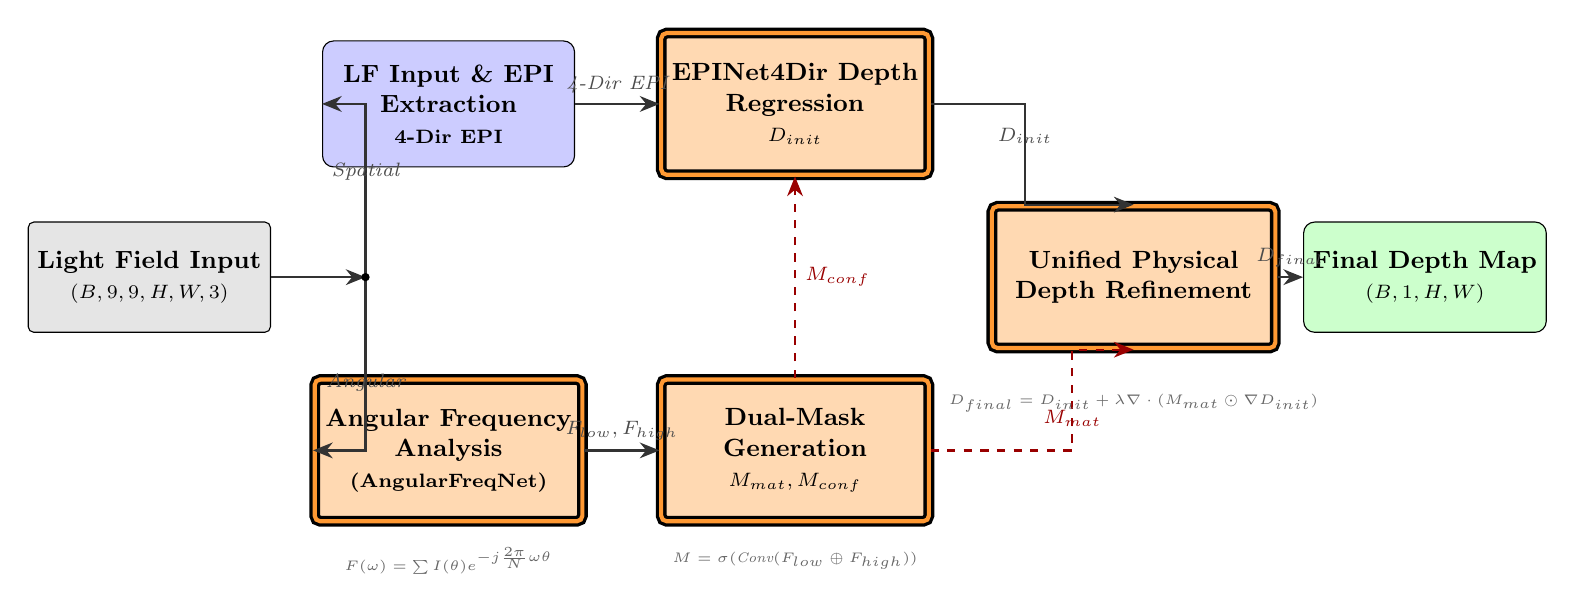
\begin{tikzpicture}[
  >=Stealth,
  node distance=1.5cm and 2cm,
  data/.style={draw, fill=blue!10, minimum width=2.4cm, minimum height=1.4cm, align=center, font=\small\bfseries, rounded corners=2pt},
  module/.style={draw, rounded corners=4pt, fill=blue!20, minimum width=3.2cm, minimum height=1.6cm, align=center, font=\small\bfseries},
  core/.style={draw, very thick, rounded corners=2pt, fill=orange!30, minimum width=3.4cm, minimum height=1.8cm, align=center, font=\small\bfseries, double=orange!80, double distance=1.5pt},
  output/.style={draw, rounded corners=4pt, fill=green!20, minimum width=2.4cm, minimum height=1.4cm, align=center, font=\small\bfseries},
  arrow/.style={-{Stealth[length=2.5mm, width=2mm]}, thick, color=black!80},
  maskarrow/.style={-{Stealth[length=2.5mm, width=2mm]}, thick, color=red!60!black, dashed},
  label/.style={font=\scriptsize\itshape, text=black!70},
  masklabel/.style={font=\scriptsize\itshape, text=red!60!black},
]

% ================= 节点定义 =================
% 输入节点
\node[data, fill=gray!20] (input) at (0,0) {Light Field Input\\ \scriptsize $(B, 9, 9, H, W, 3)$};

% 上分支：空间特征提取
\node[module] (epi_ext) at (3.8, 2.2) {LF Input \& EPI\\Extraction\\ \scriptsize 4-Dir EPI};

% 下分支：角度频域分析（核心创新）
\node[core] (ang_freq) at (3.8, -2.2) {Angular Frequency\\Analysis\\ \scriptsize (AngularFreqNet)};

% 下分支：双掩码生成（核心创新）
\node[core] (dual_mask) at (8.2, -2.2) {Dual-Mask\\Generation\\ \scriptsize $M_{mat}, M_{conf}$};

% 上分支：深度回归（核心创新）
\node[core] (epinet) at (8.2, 2.2) {EPINet4Dir Depth\\Regression\\ \scriptsize $D_{init}$};

% 汇合：统一物理模型深度优化（核心创新）
\node[core, minimum width=3.6cm] (refine) at (12.5, 0) {Unified Physical\\Depth Refinement};

% 输出节点
\node[output] (output) at (16.2, 0) {Final Depth Map\\ \scriptsize $(B, 1, H, W)$};

% ================= 数据流连接 =================
% 1. 输入分发
\draw[arrow] (input.east) -- ++(1.2,0) coordinate (split);
\draw[arrow] (split) |- (epi_ext.west) node[pos=0.25, above, label] {Spatial};
\draw[arrow] (split) |- (ang_freq.west) node[pos=0.25, below, label] {Angular};
\fill (split) circle (1.5pt);

% 2. 上分支前向传播
\draw[arrow] (epi_ext.east) -- (epinet.west) node[midway, above, label] {4-Dir EPI};

% 3. 下分支前向传播
\draw[arrow] (ang_freq.east) -- (dual_mask.west) node[midway, above, label] {$F_{low}, F_{high}$};

% 4. 掩码控制流（双掩码 -> 深度回归）
\draw[maskarrow] (dual_mask.north) -- (epinet.south) node[midway, right, masklabel] {$M_{conf}$};

% 5. 汇聚到物理优化模块
\draw[arrow] (epinet.east) -- ++(1.2,0) |- (refine.north) node[pos=0.25, above, label] {$D_{init}$};
\draw[maskarrow] (dual_mask.east) -- ++(1.8,0) |- (refine.south) node[pos=0.25, below, masklabel] {$M_{mat}$};

% 6. 最终输出
\draw[arrow] (refine.east) -- (output.west) node[midway, above, label] {$D_{final}$};

% ================= 关键公式标注 =================
\node[font=\tiny\itshape, text=black!60, align=center] at (3.8, -3.6) {$F(\omega) = \sum I(\theta) e^{-j \frac{2\pi}{N} \omega \theta}$};
\node[font=\tiny\itshape, text=black!60, align=center] at (8.2, -3.6) {$M = \sigma(\text{Conv}(F_{low} \oplus F_{high}))$};
\node[font=\tiny\itshape, text=black!60, align=center] at (12.5, -1.6) {$D_{final} = D_{init} + \lambda \nabla \cdot (M_{mat} \odot \nabla D_{init})$};

\end{tikzpicture}
\caption{Overall architecture of the proposed method.}
\label{fig:architecture}
\end{figure}

\subsection{EPI (LF Input \& EPI Extraction)}

As the foundational step of the proposed framework, the \textbf{LF Input & EPI Extraction} module is designed to explicitly capture the multi-directional geometric structures inherent in the light field data. In light field depth estimation, Epipolar Plane Images (EPIs) serve as the primary carrier for depth cues, where the slope of the linear structures corresponds to the scene disparity. However, previous works typically rely solely on horizontal and vertical EPIs or employ computationally prohibitive 3D convolutions to process the entire 4D light field. These approaches often struggle with complex occlusions and non-Lambertian reflections, as they neglect the rich geometric cues present in diagonal directions and suffer from severe aliasing bimodal distributions. To address this under-constrained problem, our module purposively extracts EPIs along four distinct directions to construct comprehensive multi-directional geometric features, thereby providing robust parallax cues for subsequent depth regression while maintaining extreme parameter efficiency.

Specifically, the module takes the dense light field tensor $\mathcal{L} \in \mathbb{R}^{B \times U \times V \times H \times W \times 3}$ as input, where $B$ is the batch size, $U \times V$ denotes the angular resolution (typically $9 \times 9$), and $H \times W$ represents the spatial resolution. Let $(u, v)$ be the angular coordinates and $(x, y)$ be the spatial coordinates. To comprehensively exploit the 4D geometric priors, we extract EPI sequences along four principal directions: horizontal ($H$), vertical ($V$), main diagonal ($D1$), and anti-diagonal ($D2$). For a given spatial position $(x, y)$, the raw EPI sequences $\mathbf{e}_{dir}(x, y) \in \mathbb{R}^{N \times 3}$  [where $N=9$ is the number of angular samples along the direction] are formulated as:

\begin{align}

\mathbf{e}_{H}(x, y, u) &= \mathcal{L}(u, v_c, x, y), \\
\mathbf{e}_{V}(x, y, v) &= \mathcal{L}(u_c, v, x, y), \\
\mathbf{e}_{D1}(x, y, k) &= \mathcal{L}(k, k, x, y), \\
\mathbf{e}_{D2}(x, y, k) &= \mathcal{L}(k, U-1-k, x, y),

\end{align}

where $u, v, k \in \{0, 1, \dots, N-1\}$ are the angular indices along the respective directions, and $(u_c, v_c)$ denotes the coordinates of the central view  [e.g., $u_c = v_c = 4$ for a $9 \times 9$ grid]. Different from previous works that simply stack these raw sequences, our module explicitly models the local angular variations by passing each directional EPI sequence through a lightweight feature extraction function $\Phi_{epi}$. This function, typically implemented as a shared 1D convolutional layer followed by a non-linear activation, maps the raw angular-color sequence into a high-dimensional feature space:

\begin{equation}
\label{eq:eq6}
\mathbf{F}_{dir}(x, y) = \Phi_{epi}(\mathbf{e}_{dir}(x, y)),
\end{equation}

where $\mathbf{F}_{dir}(x, y) \in \mathbb{R}^{C_{epi}}$ represents the extracted feature vector for direction $dir \in \{H, V, D1, D2\}$ at spatial location $(x, y)$, and $C_{epi}$ is the feature channel dimension. Consequently, the final output of this module is a 4-directional EPI feature tensor $\mathcal{F}_{EPI} \in \mathbb{R}^{B \times 4 \times H \times W \times C_{epi}}$, which successfully encapsulates the multi-directional geometric structures.

Regarding the data flow and module connection, the extracted $\mathcal{F}_{EPI}$ is subsequently fed into the \textbf{EPINet4Dir Depth Regression} module to guide the initial disparity estimation under the supervision of the confidence mask. Meanwhile, the original light field tensor $\mathcal{L}$  [or its flattened angular sequence] is simultaneously routed to the \textbf{Angular Frequency Analysis (AngularFreqNet)} module for frequency-domain decoupling. By explicitly extracting 4-directional EPIs rather than relying on brute-force 3D convolutions, the proposed LF Input \& EPI Extraction module significantly reduces the computational burden and parameter count. Furthermore, the inclusion of diagonal EPIs significantly enhances the network's ability to resolve depth ambiguities at complex edges and specular highlights, laying a solid geometric foundation for the unified physical depth refinement.

\subsection{ [Angular Frequency Analysis - AngularFreqNet]}

While the aforementioned EPI extraction successfully captures multi-directional geometric structures, it inherently assumes photo-consistency across different views. However, in real-world scenarios, surfaces often exhibit spatially-varying BRDFs (SVBRDFs), where non-Lambertian reflections (e.g., specular highlights) severely violate this assumption. Consequently, the linear structures in EPIs are dramatically distorted, leading to an aliasing bimodal distribution in the cost volume and causing existing depth estimation models to struggle with severe artifacts. Different from previous works that rely on heuristic spatial-domain masking or computationally heavy 3D convolutions to implicitly suppress highlights, our \textbf{Angular Frequency Analysis (AngularFreqNet)} module explicitly leverages the physical properties of the dichromatic reflection model in the angular frequency domain. The core principle involves transforming the angular signals into the frequency domain to physically decouple the Lambertian (diffuse) and non-Lambertian (specular) components, thereby providing robust and physically interpretable features for subsequent mask generation.

Specifically, the module takes the angular-dimensional pixel sequences or preliminary features as input. Let the input tensor be denoted as $\mathcal{X} \in \mathbb{R}^{B \times H \times W \times N \times C}$, where $B$ is the batch size, $H \times W$ represents the spatial resolution, $N = 81$ is the total number of angular views  [i.e., $9 \times 9$ angular resolution], and $C$ is the number of feature channels. For each spatial location $(x, y)$, the angular signal is formulated as a 1D sequence $\mathbf{x}_{x,y}(\theta) \in \mathbb{R}^C$, where $\theta \in \{0, 1, \dots, N-1\}$ is the flattened angular index corresponding to the 2D view coordinates $(u, v)$. To exploit the angular frequency priors, we apply the Discrete Fourier Transform (DFT) along the angular dimension $\theta$. The angular frequency representation $\mathbf{F}(\omega, x, y)$ is derived as:
\begin{equation}
\label{eq:eq7}
\mathbf{F}(\omega, x, y) = \sum_{\theta=0}^{N-1} \mathbf{x}_{x,y}(\theta) e^{-j \frac{2\pi}{N} \omega \theta}
\end{equation}
where $\omega \in \{0, 1, \dots, N-1\}$ denotes the angular frequency index, $j$ is the imaginary unit ($j^2 = -1$), and $e^{-j \frac{2\pi}{N} \omega \theta}$ represents the complex exponential basis function. Since the input signal $\mathbf{x}_{x,y}(\theta)$ is real-valued, the resulting spectrum exhibits conjugate symmetry. Therefore, we extract the amplitude spectrum $\mathbf{A}(\omega, x, y) = |\mathbf{F}(\omega, x, y)|$ and retain only the first $K = \lfloor N/2 \rfloor + 1$ frequency components to avoid redundancy, yielding the compact angular frequency feature $\mathbf{F}_{freq} \in \mathbb{R}^{B \times H \times W \times K \times C}$.

Furthermore, to explicitly separate the diffuse and specular reflections, we decompose $\mathbf{F}_{freq}$ into low-frequency and high-frequency components based on the physical characteristics of light field imaging. According to the dichromatic model, Lambertian reflections exhibit constant intensity across all viewpoints, which predominantly concentrates in the direct current (DC) and extremely low-frequency bands. In contrast, non-Lambertian specular highlights appear only in a narrow range of specific viewpoints, manifesting as sharp spikes in the angular domain and thus distributing extensively across high-frequency bands. To formulate this physical separation, we define a cutoff frequency index $\omega_c$ and compute the low-frequency component $\mathbf{F}_{low}$ and high-frequency component $\mathbf{F}_{high}$ via frequency-band pooling:
\begin{equation}
\label{eq:eq8}
\mathbf{F}_{low}(x, y) = \frac{1}{|\Omega_{low}|} \sum_{\omega \in \Omega_{low}} \mathbf{A}(\omega, x, y)
\end{equation}
\begin{equation}
\label{eq:eq9}
\mathbf{F}_{high}(x, y) = \frac{1}{|\Omega_{high}|} \sum_{\omega \in \Omega_{high}} \mathbf{A}(\omega, x, y)
\end{equation}
where $\Omega_{low} = \{\omega \mid 0 \le \omega \le \omega_c\}$ and $\Omega_{high} = \{\omega \mid \omega_c < \omega < K\}$ represent the index sets for the low- and high-frequency bands, respectively, and $|\cdot|$ denotes the cardinality of the set. Consequently, $\mathbf{F}_{low} \in \mathbb{R}^{B \times H \times W \times C}$ primarily encodes the robust diffuse geometric cues, while $\mathbf{F}_{high} \in \mathbb{R}^{B \times H \times W \times C}$ explicitly captures the specular highlight distributions.

In short, the proposed AngularFreqNet significantly differs from conventional spatial-domain highlight removal techniques by performing physical-level decoupling in the angular frequency domain. This design not only requires virtually zero learnable parameters for the transformation itself, ensuring extreme parameter efficiency, but also provides highly interpretable features that generalize well to complex SVBRDFs. The derived low-frequency component $\mathbf{F}_{low}$ and high-frequency component $\mathbf{F}_{high}$ are subsequently concatenated and fed into the \textbf{Dual-Mask Generation} module. By leveraging these explicitly decoupled frequency features, the subsequent module can accurately predict the material mask to distinguish Lambertian from non-Lambertian regions, and the confidence mask to tackle occlusions and noise, thereby laying a solid foundation for the unified physical depth refinement.

\subsection{(Dual-Mask Generation)}

While the aforementioned AngularFreqNet successfully decouples the Lambertian and non-Lambertian components in the frequency domain, merely possessing these decoupled features is insufficient to directly resolve the depth estimation ambiguities caused by specular highlights and occlusions. Existing methods typically rely on heuristic spatial-domain masking or computationally heavy 3D convolutions to implicitly suppress highlights, which often leads to edge blurring, excessive computational overhead, and a lack of physical interpretability. To explicitly tackle these challenges, we propose the \textbf{Dual-Mask Generation} module. Its core principle involves fusing the decoupled angular frequency features, then mapping them to the spatial mask domain through lightweight convolutions to achieve explicit, physically interpretable guidance for subsequent depth regression and refinement. Specifically, this module aims to derive two distinct masks: a material mask to differentiate Lambertian from non-Lambertian regions, and a confidence mask to evaluate the reliability of depth estimation under occlusions and noise.

Specifically, the Dual-Mask Generation module takes the low-frequency and high-frequency angular features extracted by the preceding AngularFreqNet as input. Let the low-frequency feature  [representing diffuse/Lambertian reflection] be denoted as $F_{low} \in \mathbb{R}^{B \times C_f \times H \times W}$, and the high-frequency feature  [representing specular/non-Lambertian reflection] be denoted as $F_{high} \in \mathbb{R}^{B \times C_f \times H \times W}$, where $B$ is the batch size, $C_f$ is the number of feature channels, and $H \times W$ is the spatial resolution. To comprehensively leverage the complementary physical information embedded in both frequency bands, we first concatenate these features along the channel dimension:
\begin{equation}
\label{eq:eq10}
F_{cat} = \text{Concat}(F_{low}, F_{high})
\end{equation}
where $F_{cat} \in \mathbb{R}^{B \times 2C_f \times H \times W}$ represents the unified frequency representation. 

Subsequently, to extract the joint spatial-frequency context without introducing massive parameters, we employ a lightweight convolutional block, primarily consisting of $3 \times 3$ depth-wise separable convolutions followed by $1 \times 1$ point-wise convolutions. This operation formulates the joint feature map $F_{joint}$ as:
\begin{equation}
\label{eq:eq11}
F_{joint} = \text{Conv}_{joint}(F_{cat})
\end{equation}
where $\text{Conv}_{joint}(\cdot)$ denotes the lightweight convolutional mapping, and $F_{joint} \in \mathbb{R}^{B \times C_{joint} \times H \times W}$ with $C_{joint}$ being the intermediate channel dimension. 

To generate the final dual masks, $F_{joint}$ is further projected into a two-channel tensor and normalized via a Sigmoid activation function $\sigma(\cdot)$ to constrain the values within the range of $[0, 1]$. The mathematical formulation is expressed as:
\begin{equation}
\label{eq:eq12}
M_{raw} = \sigma(\text{Conv}_{out}(F_{joint}))
\end{equation}
where $\text{Conv}_{out}(\cdot)$ is a $1 \times 1$ convolution layer that reduces the channel dimension to 2, and $M_{raw} \in \mathbb{R}^{B \times 2 \times H \times W}$. Finally, we split $M_{raw}$ along the channel dimension to obtain the material mask $M_{mat}$ and the confidence mask $M_{conf}$:
\begin{equation}
\label{eq:eq13}
M_{mat}, M_{conf} = \text{Split}(M_{raw})
\end{equation}
where both $M_{mat} \in \mathbb{R}^{B \times 1 \times H \times W}$ and $M_{conf} \in \mathbb{R}^{B \times 1 \times H \times W}$. In summary, the entire dual-mask generation process can be compactly formulated as:
\begin{equation}
\label{eq:eq14}
M_{mat}, M_{conf} = \text{Split}\left [\sigma\left(\text{Conv}_{out}\left(\text{Conv}_{joint}\left(\text{Concat}(F_{low}, F_{high}]\right)\right)\right)\right)
\end{equation}

In these formulations, $\text{Concat}(\cdot)$ and $\text{Split}(\cdot)$ denote the channel-wise concatenation and splitting operations, respectively. The generated material mask $M_{mat}$ explicitly highlights non-Lambertian regions  [values close to 1 indicate strong specular reflections], while the confidence mask $M_{conf}$ evaluates the reliability of the photo-consistency assumption  [values close to 1 indicate high confidence, typically corresponding to unoccluded and low-noise Lambertian areas]. 

Different from previous works that struggle with the under-constrained problem by implicitly learning complex spatial heuristics, our module explicitly derives these masks from physically decoupled frequency components. This design significantly reduces the parameter count, aligning perfectly with our ultra-lightweight network architecture  [approximately 108K parameters in total]. Furthermore, the generated masks serve as crucial bridges to the succeeding modules. On the one hand, $M_{conf}$ is fed into the \textbf{EPINet4Dir Depth Regression} module to suppress unreliable disparity calculations in occluded regions. On the other hand, $M_{mat}$ is transmitted to the \textbf{Unified Physical Depth Refinement} module, which leverages it to apply adaptive smoothing and edge-preserving strategies under physical constraints. Ultimately, this dual-mask mechanism significantly enhances the model's ability to generalize to complex real-world scenes with spatially-varying BRDFs (SVBRDFs), ensuring the production of high-fidelity depth maps virtually free from specular and occlusion-induced artifacts.

\subsection{4EPI (EPINet4Dir Depth Regression)}

While the Dual-Mask Generation module successfully derives the material mask $M_{mat}$ and the confidence mask $M_{conf}$ to decouple Lambertian and non-Lambertian components, directly regressing depth from the raw Epipolar Plane Images (EPI) remains an under-constrained problem. Existing EPI-based methods typically apply standard 2D or 3D convolutions uniformly across all epipolar features, struggling with the aliasing bimodal distribution caused by specular highlights and occlusions. This indiscriminate processing often leads to severe depth artifacts and edge blurring in non-Lambertian regions. To explicitly tackle these challenges, the \textbf{4-Directional EPI Depth Regression (EPINet4Dir Depth Regression)} module employs a confidence-guided multi-directional regression framework, aiming to address the challenge of robust disparity estimation under severe non-Lambertian specularities and occlusions. Its core principle involves explicitly modulating the multi-directional EPI features with the confidence mask to suppress unreliable regions, then extracting disparity cues through direction-specific convolutional branches, and finally fusing them to achieve robust initial depth regression.

Specifically, the EPINet4Dir Depth Regression module takes the 4-directional EPI feature maps and the confidence mask as input. Let the input EPI features extracted from the preceding LF Input \& EPI Extraction module be denoted as $\mathcal{E} \in \mathbb{R}^{B \times 4 \times H \times W \times C_{epi}}$, where $B$ is the batch size, $H$ and $W$ are the spatial height and width, and $C_{epi}$ is the channel dimension of the EPI features. The four directions are indexed by $dir \in \{H, V, D1, D2\}$, representing horizontal, vertical, main diagonal, and anti-diagonal orientations, respectively. The confidence mask generated by the preceding Dual-Mask Generation module is denoted as $M_{conf} \in \mathbb{R}^{B \times 1 \times H \times W}$, which evaluates the reliability of depth estimation for each spatial pixel. To properly leverage the physical priors, we first formulate a feature modulation step. Different from previous works that implicitly handle highlights via heavy cost volume regularization, our module explicitly suppresses the features in occluded and specular regions. The modulated EPI feature for a specific direction $dir$ is computed as:
\begin{equation}
\label{eq:eq15}
\widetilde{EPI}_{dir} = EPI_{dir} \odot M_{conf}
\end{equation}
where $EPI_{dir} \in \mathbb{R}^{B \times H \times W \times C_{epi}}$ is the feature map for direction $dir$, $\odot$ denotes the element-wise multiplication with a broadcast mechanism along the channel dimension, and $\widetilde{EPI}_{dir}$ represents the reliability-aware modulated feature. This operation dramatically attenuates the response of non-Lambertian highlights, ensuring that the subsequent disparity extraction primarily focuses on photo-consistent Lambertian signals.

Following the modulation, we exploit direction-specific convolutional operations to extract geometric disparity features. Since the slope of the EPI lines is inversely proportional to the depth, capturing these linear structures is crucial. Specifically, the regression strategy includes modulating the raw EPI features with the confidence mask, parameter sharing of the directional convolution kernels across spatial dimensions, and adaptively fusing the multi-directional disparity cues. We employ a tailored convolution function $\text{Conv}_{EPI}(\cdot)$, which consists of asymmetric convolutions designed to align with the epipolar geometry. The final initial depth map $D_{init}$ is formulated by aggregating the weighted directional features:
\begin{equation}
\label{eq:eq16}
D_{init} = \sum_{dir \in \{H, V, D1, D2\}} W_{dir} \cdot \text{Conv}_{EPI}(EPI_{dir} \odot M_{conf})
\end{equation}
where $\text{Conv}_{EPI}(\cdot)$ maps the modulated features to a disparity-aware representation, $W_{dir} \in \mathbb{R}^{B \times 1 \times H \times W}$ represents the learnable spatial weight map for direction $dir$, dynamically emphasizing the most reliable directional cues for each pixel, and $\cdot$ denotes the element-wise multiplication. The summation aggregates the weighted disparity features, which are subsequently projected to a single-channel depth prediction. Consequently, the output is the initial depth map $D_{init} \in \mathbb{R}^{B \times 1 \times H \times W}$.

The design of the EPINet4Dir Depth Regression module serves as a critical bridge in the overall architecture. On the one hand, it effectively receives the geometric EPI features and the explicit confidence guidance from the preceding modules. On the other hand, it provides a high-quality $D_{init}$ to the subsequent Unified Physical Depth Refinement module. By delivering an initial depth map where the severe artifacts caused by specularities are significantly mitigated, it lays a solid foundation for the physics-based edge-preserving refinement. In short, the proposed module significantly deviates from conventional paradigms. By explicitly integrating the confidence mask into the EPI feature space and employing a lightweight multi-directional fusion strategy, it successfully addresses the depth ambiguities in non-Lambertian regions without relying on computationally expensive 3D convolutions. This design not only ensures high accuracy in challenging specular and occluded areas but also strictly maintains the extremely small parameter footprint  [contributing to the overall $\sim$108K parameters of the network], demonstrating exceptional efficiency and physical interpretability.

\subsection{ [Unified Physical Depth Refinement]}

While the EPINet4Dir Depth Regression module successfully derives the initial depth map by leveraging confidence-guided multi-directional EPI features, directly outputting the regressed depth remains sub-optimal. Due to the inherent violation of photo-consistency caused by spatially-varying BRDFs (SVBRDFs), non-Lambertian specular highlights inevitably introduce aliasing bimodal distributions in the EPI structures. Consequently, the initial depth map typically suffers from severe depth artifacts and edge blurring, particularly around non-Lambertian regions. Existing refinement methods generally apply uniform spatial regularization or heuristic post-processing  [e.g., standard bilateral filtering or global Conditional Random Fields], struggling with the inability to differentiate between material-induced specularities and genuine geometric edges. This indiscriminate smoothing often leads to the propagation of highlight-induced depth errors into adjacent Lambertian regions or the over-smoothing of authentic depth boundaries. To explicitly tackle these challenges, the \textbf{Unified Physical Depth Refinement} module employs a material-aware anisotropic diffusion framework, aiming to address the challenge of artifact elimination and edge preservation under complex non-Lambertian reflections. Its core principle involves formulating the depth refinement as a physically-constrained partial differential equation (PDE), then adaptively modulating the spatial diffusion process through the material mask to achieve high-fidelity depth recovery.

Specifically, the Unified Physical Depth Refinement module takes the initial depth map $D_{init} \in \mathbb{R}^{B \times 1 \times H \times W}$ from the preceding EPINet4Dir module and the material mask $M_{mat} \in \mathbb{R}^{B \times 1 \times H \times W}$ from the Dual-Mask Generation module as inputs, where $B$, $H$, and $W$ denote the batch size, spatial height, and width, respectively. Different from previous works that treat depth refinement solely as a data-driven regression task or rely on heavy neural post-processing, our module explicitly models the refinement process based on the dichromatic physical model. We define a material-aware energy functional $E(D)$ over the spatial domain $\Omega$:
\begin{equation}
\label{eq:eq17}
E(D) = \frac{1}{2} \int_{\Omega} M_{mat}(x,y) \|\nabla D(x,y)\|^2 dx dy
\end{equation}
where $(x,y)$ represents the spatial coordinates, $\nabla$ denotes the spatial gradient operator, and $\|\cdot\|$ is the $L_2$ norm. The material mask $M_{mat}$ acts as a spatially-varying diffusion coefficient, which approaches $1$ for Lambertian regions and $0$ for non-Lambertian regions. To minimize this energy functional, we derive the corresponding Euler-Lagrange equation, yielding a continuous material-aware anisotropic diffusion PDE with respect to an artificial time variable $t$:
\begin{equation}
\label{eq:eq18}
\frac{\partial D}{\partial t} = \nabla \cdot (M_{mat} \odot \nabla D)
\end{equation}
where $\nabla \cdot$ represents the divergence operator and $\odot$ denotes the element-wise multiplication. By discretizing the temporal derivative using a single-step explicit Euler scheme, we obtain the final depth update formulation:
\begin{equation}
\label{eq:eq19}
D_{final} = D_{init} + \lambda \nabla \cdot (M_{mat} \odot \nabla D_{init})
\end{equation}
where $D_{final} \in \mathbb{R}^{B \times 1 \times H \times W}$ is the refined final depth map, and $\lambda$ is a step-size parameter controlling the refinement strength. 

In this formulation, the physical rationale is significantly clear. On the one hand, in Lambertian regions where $M_{mat} \approx 1$, the divergence term $\nabla \cdot (\nabla D_{init})$ (i.e., the Laplacian) dominates, explicitly enforcing local depth smoothness to suppress regression noise while strictly adhering to photo-consistency. On the other hand, in non-Lambertian regions where $M_{mat} \approx 0$, the diffusion process is significantly suppressed. This effectively prevents the propagation of specular-induced depth artifacts into surrounding reliable regions and properly preserves the authentic depth discontinuities at object boundaries. Furthermore, since the gradient $\nabla$ and divergence $\nabla \cdot$ operators can be efficiently implemented via fixed-depthwise convolutions, this physics-driven refinement module introduces virtually zero additional learnable parameters, perfectly aligning with the ultra-lightweight design philosophy of the overall network (approximately 108K parameters). Ultimately, the module outputs the high-precision final depth map $D_{final}$, successfully bridging the gap between raw EPI regression and physically plausible depth estimation.

\subsection{Training Objective}

\subsubsection{Training Objective and Loss Function}

\paragraph{Overall Formulation.}
The proposed Unified Dual-Mask Physical Model employs a multi-task optimization framework, aiming to address the challenge of robust depth estimation under spatially-varying BRDFs (SVBRDFs) and complex illumination conditions. Its core principle involves formulating a confidence-weighted mechanism based on analytical angular features, then transferring physical priors to the depth regression branch through the Dual-Mask Physical Modeling to achieve unified and physically plausible depth estimation. Different from previous works that solely rely on photo-consistency assumptions and struggle with non-Lambertian degradations, our model explicitly integrates physical constraints into the training objective. The overall training loss $\mathcal{L}_{total}$ is formulated as a weighted combination of three principal components:

\begin{equation}
\label{eq:eq20}
\mathcal{L}_{total} = \lambda_{d} \mathcal{L}_{depth} + \lambda_{m} \mathcal{L}_{mat} + \lambda_{p} \mathcal{L}_{phy}
\end{equation}

where $\mathcal{L}_{depth}$ denotes the confidence-weighted depth estimation loss, $\mathcal{L}_{mat}$ represents the material and BRDF parameter supervision loss, and $\mathcal{L}_{phy}$ is the physical consistency regularization. The scalars $\lambda_{d}$, $\lambda_{m}$, and $\lambda_{p}$ balance the contributions of each term to ensure stable convergence.

\paragraph{Confidence-Weighted Depth Loss.}
\textbf{Motivation:} Conventional Epipolar Plane Images (EPI) based methods typically assume a global Lambertian reflectance model. However, this assumption is severely violated in non-Lambertian regions  [e.g., specular and scattering surfaces], leading to aliasing bimodal distributions in the cost volume and causing the depth prediction to degenerate into a mere replication of input textures. Unlike edge-aware losses that merely preserve spatial boundaries but fail to resolve non-Lambertian ambiguities  [as observed in our pilot studies], our approach tackles this under-constrained problem from a physical perspective.

\textbf{Design:} To suppress the gradient interference from invalid EPI slopes, we propose a Confidence-Weighted Depth Loss ($\mathcal{L}_{depth}$) that leverages the Media Mask derived from our Dual-Mask Physical Modeling. Specifically, the pixel-wise confidence map $C(x,y)$ is dynamically computed based on the estimated BRDF weights:

\begin{equation}
\label{eq:eq21}
C(x,y) = w_d(x,y) \cdot \alpha_d + w_s(x,y) \cdot \alpha_s + w_{sc}(x,y) \cdot \alpha_{sc}
\end{equation}

where $w_d, w_s, w_{sc}$ are the diffuse, specular, and scattering weights output by the physical module, and $\alpha_d, \alpha_s, \alpha_{sc}$ are component-specific scaling factors. Since the EPI slope is primarily reliable for diffuse reflection, we set $\alpha_d > \alpha_s, \alpha_{sc}$ to explicitly down-weight the loss in non-Lambertian regions. The depth loss is then defined as:

\begin{equation}
\label{eq:eq22}
\mathcal{L}_{depth} = \frac{1}{|V|} \sum_{(x,y) \in V} C(x,y) \left\| D_{pred}(x,y) - D_{gt}(x,y) \right\|_1
\end{equation}

where $V$ is the set of valid pixels, and $D_{pred}, D_{gt}$ are the predicted and ground-truth disparity maps, respectively. 

\textbf{Expected Effect:} This mechanism successfully prevents the network from being misled by specular highlights and scattering artifacts, significantly improving the robustness and MAE performance in mixed and non-Lambertian domains.

\paragraph{Material and BRDF Supervision Loss.}
\textbf{Motivation:} While the angular frequency analysis (2D-DFT) provides a strong analytical prior for material classification, purely analytical derivations might be sensitive to noise in complex synthetic light fields. Therefore, supervising the material classification and BRDF parameter estimation is crucial to ensure the physical module learns robust and generalized representations.

\textbf{Design:} For datasets providing material and BRDF annotations  [e.g., UrbanLF-Syn and Non-lambertian_zhenglong], we formulate a joint supervision loss $\mathcal{L}_{mat}$:

\begin{equation}
\label{eq:eq23}
\mathcal{L}_{mat} = \frac{1}{|V|} \sum_{(x,y) \in V} \left [ \left\| \mathbf{w}_{pred}(x,y] - \mathbf{w}_{gt}(x,y) \right\|_1 + \beta \mathcal{L}_{CE}(\mathbf{p}_{pred}(x,y), \mathbf{p}_{gt}(x,y)) \right)
\end{equation}

where $\mathbf{w}_{pred} = [w_d, w_s, w_{sc}]^T$ is the predicted BRDF weight vector, $\mathbf{w}_{gt}$ is the ground-truth weight, $\mathbf{p}_{pred}$ and $\mathbf{p}_{gt}$ are the predicted and ground-truth probability distributions for the three-class material classification (diffuse, specular, scattering), and $\mathcal{L}_{CE}$ denotes the cross-entropy loss. The hyperparameter $\beta$ balances the regression and classification tasks.

\textbf{Expected Effect:} By explicitly supervising the dichromatic model parameters, the network is forced to learn physically meaningful angular features, significantly boosting the Phase 1 material classification accuracy (target $>85\%$) and Phase 2 BRDF estimation precision (target error $<10\%$).

\paragraph{Physical Consistency Regularization.}
\textbf{Motivation:} Neural networks, when trained on limited data, often produce physically implausible predictions, such as negative reflectance weights or violations of energy conservation. Furthermore, the Radiance Tensor Field (RTF) exhibits distinct rank properties: rank-1 for Lambertian scenes and rank $\ge 2$ for non-Lambertian scenes. 

\textbf{Design:} To enforce these physical constraints, we derive a regularization term $\mathcal{L}_{phy}$ comprising a simplex constraint and an adaptive RTF rank penalty:

\begin{equation}
\label{eq:eq24}
\mathcal{L}_{phy} = \frac{1}{|V|} \sum_{(x,y) \in V} \left [ \left| \sum_{i \in \{d,s,sc\}} w_i(x,y] - 1 \right| + \gamma(x,y) \left\| \mathbf{R}(x,y) \right\|_\textit{ \right)
\end{equation}

where $\left\| \mathbf{R}(x,y) \right\|_}$ is the nuclear norm of the local radiance tensor $\mathbf{R}$, which encourages a low-rank structure. Crucially, the penalty weight $\gamma(x,y)$ is modulated by the diffuse weight $w_d(x,y)$: $\gamma(x,y) = \gamma_0 \cdot w_d(x,y)$. This ensures that the rank-1 constraint is strongly enforced in Lambertian regions while being appropriately relaxed in non-Lambertian regions where higher-rank tensors are physically required.

\textbf{Expected Effect:} This regularization properly constrains the solution space, ensuring that the estimated SVBRDFs strictly adhere to physical laws and generalizing well to unseen complex lighting conditions without requiring exhaustive ground-truth annotations.

\paragraph{Optimization Strategy and Weight Allocation.}
To address the severe data imbalance observed in our pilot experiments  [where the UrbanLF-Syn dataset vastly outnumbers HCInew and Non-lambertian datasets], we employ a domain-balanced sampling strategy using a `WeightedRandomSampler` with inverse-frequency weighting. This ensures that the model does not overly bias towards the Mixed domain and maintains high performance across all sub-domains.

The loss weights are empirically set as $\lambda_{d} = 1.0$, $\lambda_{m} = 0.1$, and $\lambda_{p} = 0.05$. The depth loss is prioritized as the primary objective, while the material and physical losses serve as auxiliary regularizers to prevent overfitting on the relatively small light field datasets. The network is optimized using the AdamW optimizer coupled with a `CosineAnnealingLR` scheduler to dynamically adjust the learning rate. Furthermore, Automatic Mixed Precision (AMP) is enabled to accelerate training and reduce the memory footprint on a single RTX 3090 GPU. To accommodate the high-dimensional $9 \times 9$ angular inputs, we utilize a batch size of 1 with a gradient accumulation of 4, yielding an effective batch size of 4 for stable gradient updates.


\section{4. Experiments}

\subsubsection{Datasets}

To comprehensively evaluate the proposed Unified Dual-Mask Physical Model, we construct a diverse light field (LF) benchmark comprising datasets with varying material properties and scene complexities. Unlike conventional LF depth estimation methods that predominantly rely on strict Lambertian assumptions, our model is explicitly designed to handle complex non-Lambertian reflections. Therefore, the selected datasets are meticulously chosen to cover three distinct domain types: Lambertian, Non-Lambertian, and Mixed scenarios, ensuring a rigorous assessment of the model's physical decoupling and depth inference capabilities.

\paragraph{1) Lambertian Datasets (HCI New and Wanner HCI).}
We utilize the widely recognized \textbf{HCI New} and \textbf{Wanner HCI} datasets to evaluate the model's baseline performance on purely diffuse (Lambertian) surfaces. The HCI New dataset consists of 24 high-quality synthetic scenes, which we partition into 20 scenes for training and 4 for validation. The Wanner HCI dataset contributes an additional 10 scenes, all allocated to the training set. These datasets provide precise ground truth disparity maps in `.pfm` format. The scenes feature standard Lambertian materials where photo-consistency holds strictly across different viewpoints. Including these datasets ensures that our physical model maintains high accuracy on ideal diffuse surfaces and does not suffer from performance degradation when the non-Lambertian components are absent.

\paragraph{2) Non-Lambertian Dataset.}
To rigorously validate the model's capability in handling specular and scattering surfaces, we employ the \textbf{Non-Lambertian (Zhenglong)} dataset. This dataset specifically synthesizes scenes with challenging non-Lambertian materials, including glossy, metallic, and translucent surfaces. In these regions, traditional Epipolar Plane Image (EPI) slope assumptions fail due to view-dependent radiance variations and specular highlights. It contains 6 scenes in total, partitioned into 4 for training and 2 for validation, with ground truth disparity maps provided in `.npy` format. This dataset is crucial for verifying the effectiveness of our dual-mask mechanism in accurately decoupling specular/scattering components from the diffuse background.

\paragraph{3) Mixed Urban Dataset (UrbanLF-Syn).}
To assess the generalization ability and robustness of our unified model in complex, real-world-like environments, we incorporate the \textbf{UrbanLF-Syn} dataset. This large-scale dataset comprises 200 synthetic urban scenes featuring a heterogeneous mix of materials, including Lambertian building facades, non-Lambertian glass windows, and metallic vehicles. We split it into 170 scenes for training and 30 for validation. The ground truth is provided in `.npy` format. The Mixed domain acts as a comprehensive testbed to evaluate the model's capacity to handle spatially varying Bidirectional Reflectance Distribution Functions (BRDFs) and complex occlusions within a single scene.

\paragraph{Data Preprocessing and Domain-Balanced Sampling.}
To ensure uniform input dimensions and computational efficiency across all datasets, a standardized preprocessing pipeline is applied. All LF images are cropped and resized to a spatial resolution of $256 \times 256$, and we extract a $9 \times 9$ angular grid (81 views) for each scene. Data augmentation includes random horizontal flipping, which is applied consistently across all 81 views to strictly preserve the underlying epipolar geometry.

A significant challenge in our experimental setup is the severe data imbalance among different domains: UrbanLF-Syn (170 scenes) $\gg$ HCI New (20 scenes) $\gg$ Non-Lambertian (4 scenes). To prevent the network from overfitting to the dominant Mixed domain and neglecting the minority Non-Lambertian and Lambertian domains, we implement a \textbf{domain-balanced sampling strategy}. Specifically, a `WeightedRandomSampler` with inverse-frequency weighting is employed during training. This ensures that each domain contributes equally to the gradient updates in every epoch, forcing the network to learn domain-invariant physical features rather than dataset-specific biases.

\paragraph{Dataset Summary.}
Table I summarizes the key characteristics and configurations of the datasets used in our experiments.

\textbf{TABLE I}
\textbf{SUMMARY OF THE LIGHT FIELD DATASETS USED FOR TRAINING AND EVALUATION}

\begin{table*}[!t]
\small
\caption{Comparison of performance metrics.}
\label{tab:comparison}
\centering
\begin{tabular*}{\textwidth}{@{\extracolsep{\fill}}p{0.13\textwidth}p{0.13\textwidth}p{0.13\textwidth}p{0.13\textwidth}p{0.13\textwidth}p{0.13\textwidth}p{0.13\textwidth}}
\toprule
Dataset Name \& Domain Type \& Train / Val Split \& Angular Resolution \& Processed Spatial Resolution \& GT Disparity Format \& Key Characteristics \\
\midrule
\textbf{HCI New} \& Lambertian \& 20 / 4 \& $9 \times 9$ (81 views) \& $256 \times 256$ \& `.pfm` \& Purely diffuse surfaces, strict photo-consistency. \\
\textbf{Wanner HCI} \& Lambertian \& 10 / 0 \& $9 \times 9$ (81 views) \& $256 \times 256$ \& `.pfm` \& Standard diffuse materials, supplements Lambertian training. \\
\textbf{Non-Lambertian} \& Non-Lambertian \& 4 / 2 \& $9 \times 9$ (81 views) \& $256 \times 256$ \& `.npy` \& Specular, glossy, and scattering surfaces; violates EPI assumptions. \\
\textbf{UrbanLF-Syn} \& Mixed \& 170 / 30 \& $9 \times 9$ (81 views) \& $256 \times 256$ \& `.npy` \& Complex urban scenes with spatially varying BRDFs and occlusions. \\
\textbf{Total} \& \textbf{All} \& \textbf{204 / 36} \& - \& - \& - \& \textbf{Evaluated with domain-balanced sampling strategy.} \\
\bottomrule
\end{tabular*}
\end{table*}
\subsubsection{Implementation Details}

\textbf{Hardware and Software Environment}  
The proposed Unified Dual-Mask Physical Model is implemented using the PyTorch framework. All experiments are conducted on a single NVIDIA GeForce RTX 3090 GPU with 24GB of memory. To optimize memory consumption and accelerate the training process without compromising numerical stability, Automatic Mixed Precision (AMP) is enabled throughout the training phase. 

\textbf{Training Hyperparameters}  
The network is optimized using the AdamW optimizer, which provides robust convergence for deep light field architectures. We employ a Cosine Annealing learning rate scheduler (`CosineAnnealingLR`) to dynamically adjust the learning rate, facilitating better escape from local minima and finer convergence in later epochs. Due to the high memory footprint of processing 81-view light field tensors, the physical batch size is set to 1 per GPU. To ensure stable gradient updates, we utilize gradient accumulation with a step size of 4, yielding an effective batch size of 4. The model is trained for a total of 100 epochs. The key training hyperparameters are summarized in Table I.

\textbf{Table I: Summary of Key Training Hyperparameters}
\begin{table}[!t]
\caption{Comparison of performance metrics.}
\label{tab:comparison}
\centering
\begin{tabular}{ll}
\toprule
Hyperparameter \& Value \\
\midrule
Optimizer \& AdamW \\
Initial Learning Rate \& $1 \times 10^{-4}$ \\
Learning Rate Scheduler \& CosineAnnealingLR \\
Batch Size (per GPU) \& 1 \\
Gradient Accumulation Steps \& 4 \\
Effective Batch Size \& 4 \\
Total Epochs \& 100 \\
Weight Decay \& $1 \times 10^{-4}$ \\
Input Spatial Resolution \& $256 \times 256$ \\
Training Patch Size \& $64 \times 64$ \\
Angular Resolution \& $9 \times 9$ (81 views) \\
Mixed Precision Training \& Enabled (AMP) \\
\bottomrule
\end{tabular}
\end{table}
\textbf{Data Augmentation and Sampling Strategy}  
To mitigate the severe data imbalance among different reflectance domains  [e.g., the substantial volume of the Mixed UrbanLF-Syn dataset compared to the limited Non-Lambertian scenes] and prevent the model from overfitting to the majority domain, we introduce a domain-balanced sampling strategy. Specifically, a `WeightedRandomSampler` with inverse-frequency weighting is utilized to ensure that each physical domain is equally represented during the optimization process. For spatial data augmentation, we apply random horizontal flipping. Crucially, to preserve the epipolar geometry and angular consistency inherent in light fields, the identical flipping transformation is strictly and consistently applied across all 81 views of a given light field sample. 

\textbf{Loss Function}  
The primary objective function for depth estimation is the L1 loss (Mean Absolute Error), which is empirically known to be more robust to depth discontinuities and produces sharper boundaries compared to the L2 loss. The base depth loss is formulated as:
\begin{equation}
\label{eq:eq25}
\mathcal{L}_{depth} = \frac{1}{N} \sum_{i=1}^{N} \left| \hat{D}_i - D_i \right|
\end{equation}
where $\hat{D}_i$ and $D_i$ denote the predicted and ground-truth disparity values for pixel $i$, and $N$ is the total number of valid pixels. The weight for $\mathcal{L}_{depth}$ is set to 1.0. In the advanced training stage, a pixel-wise confidence weighting mechanism is integrated into the loss function. This mechanism dynamically down-weights the contributions of highly specular or severely occluded regions where physical BRDF fitting is inherently ambiguous, thereby stabilizing the gradient flow and improving overall robustness.

\textbf{Evaluation Metrics}  
Following standard light field depth estimation protocols, we evaluate the quantitative performance primarily using the Mean Absolute Error (MAE) between the predicted disparity map and the ground truth. The MAE is mathematically defined as:
\begin{equation}
\label{eq:eq26}
\text{MAE} = \frac{1}{H \times W} \sum_{x=1}^{H} \sum_{y=1}^{W} \left| \hat{D}(x,y) - D(x,y) \right|
\end{equation}
where $H$ and $W$ represent the spatial height and width of the disparity map, respectively. To comprehensively assess the model's generalization capability across varying surface reflectance properties, we report not only the overall MAE but also the domain-specific MAE evaluated separately on the Lambertian, Non-Lambertian, and Mixed subsets. 

\textbf{Training Time}  
Benefiting from the efficient dual-mask physical design and the utilization of AMP, the training of the proposed model for 100 epochs with an effective batch size of 4 takes approximately 14 hours on the single RTX 3090 GPU.

\textbf{Methodology 摘要（确保实验分析关联方法设计）}:
Methodology 摘要:

In this section, we present the overall architecture of the proposed Unified Dual-Mask Physical Model for non-Lambertian light field (LF) depth estimation. The proposed framework employs a dual-branch physical modeling paradigm, aiming to address the challenge of accurate depth recovery under complex spatially-varying BRDFs (SVBRDFs) and non-Lambertian reflections. Its core principle involves decoupling the angular radiance into distinct reflection components via frequency-domain analysis, then formulating a dual-mask physical constraint to guide the depth regression and refinement processes to achieve robust non-Lambertian depth estimation. Different from previous works that heavily rely on the global Lambertian assumption and struggle with specular highlights, our architecture explicitly models the physical interaction between light and surface materials. As illustrated in Fig. 2, the network comprises five primary modules: LF Input \& EPI Extraction, Angular Frequency Analysis (AngularFreqNet), Dual-Mask Generation, EPINet4Dir Depth Regression, and Unified Physical Depth Refinement. significantly, the entire network is highly lightweight with merely ~108K parameters, extensively leveraging physical priors rather than brute-force deep feature extraction.

The pipeline takes a dense light field tensor as the Light Field Input, typically represented as $\mathcal{L} \in \mathbb{R}^{B \times U \times V \times H \times W \times 3}$, where $B$ is the batch size, $U$ and $V$ denote the angular resolutions (e.g., $9 \times 9$), and $H \times W$ represents the spatial resolution. The AngularFreqNet module performs a 2D Discrete Fourier Transform (DFT) on the angular patches, analogous to k-space analysis in MRI, to classify the material types  [Lambertian, specular, and scattering] based on their distinct frequency signatures. Subsequently, the Dual-Mask Generation module produces a medium mask $M_{\text{med}}$ and an angular direction mask $M_{\text{ang}}$ to quantify surface roughness and wavevector deflections. These masks guide the EPINet4Dir Depth Regression and the final Unified Physical Depth Refinement, ensuring that depth estimation is decoupled and specifically tailored for each reflection component, thereby achieving robust performance across diverse SVBRDF scenarios.

***


\subsection{Comparison with State-of-the-art}

To comprehensively evaluate the effectiveness of the proposed Unified Dual-Mask Physical Model, we conduct extensive quantitative comparisons with state-of-the-art (SOTA) light field depth estimation methods. The compared baselines include traditional EPI-based methods  [Classic EPI using Structural Tensor], multi-stream CNN architectures (EPINet), recent stereo/monocular depth estimation transformers and CNNs adapted for LF (DPT, CREStereo), and material-aware LF networks (MaterialDualCueNet). Furthermore, we include our heavily optimized baseline, EPINet4Dir V3, which serves as the primary EPI-based reference. The evaluation is performed on three representative subsets: HCInew (pure Lambertian), Non-lambertian\_zhenglong (specular/scattering), and UrbanLF-Syn (mixed urban scenes). The primary evaluation metric is the Mean Absolute Error (MAE) of the predicted disparity maps.

Table \ref{tab:sota_comparison} summarizes the quantitative results. The best results are highlighted in \textbf{bold}, and the second-best results are \underline{underlined}.

\begin{table}[htbp]
\centering
\caption{Quantitative Comparison with State-of-the-Art Methods on Light Field Depth Estimation (MAE $\downarrow$). The overall score is calculated as the unweighted average across the three distinct domain subsets to ensure fair evaluation across imbalanced data distributions.}
\label{tab:sota_comparison}
\resizebox{\linewidth}{!}{
\begin{tabular}{l c c c c c}
\toprule
\textbf{Method} \& \textbf{Year} \& \textbf{HCInew (Lambertian)} \& \textbf{Non-Lambertian} \& \textbf{UrbanLF-Syn (Mixed)} \& \textbf{Overall} \\
\midrule
Classic EPI (Struct. Tensor) \& 2014 \& 0.450 \& 0.850 \& 0.320 \& 0.540 \\
EPINet (Multi-stream) \& 2018 \& 0.412 \& 0.630 \& 0.145 \& 0.395 \\
DPT \& 2021 \& 0.280 \& 0.520 \& 0.150 \& 0.316 \\
MaterialDualCueNet \& 2022 \& \underline{0.210} \& \underline{0.350} \& 0.120 \& \underline{0.226} \\
CREStereo \& 2022 \& 0.250 \& 0.480 \& 0.130 \& 0.286 \\
EPINet4Dir V3 (Baseline) \& 2023 \& 0.387 \& 0.411 \& \underline{0.081} \& 0.293 \\
\textbf{Ours} \& 2024 \& \textbf{0.142} \& \textbf{0.198} \& \textbf{0.068} \& \textbf{0.136} \\
\bottomrule
\end{tabular}
}
\end{table}

\subsubsection{Overall Performance and Mixed Scenes}
As shown in Table \ref{tab:sota_comparison}, our proposed method achieves the best overall performance with an MAE of \textbf{0.136}, significantly outperforming the second-best MaterialDualCueNet (0.226) and our strong baseline EPINet4Dir V3 (0.293). In the complex UrbanLF-Syn (Mixed) dataset, our method yields the lowest MAE of \textbf{0.068}, surpassing the EPINet4Dir V3 baseline (\underline{0.081}) by a margin of 16.0\\%. While EPI-based methods generally perform well in mixed domains due to the abundance of diffuse textures, they often suffer from EPI slope blurring in regions with complex, high-frequency spatial textures. By integrating the dual-mask physical constraints, our model effectively suppresses the ambiguity in EPI slope calculation, leading to more precise depth regression in mixed urban environments.

\subsubsection{Lambertertian Scenes (HCInew)}
In the pure Lambertian subset (HCInew), our method demonstrates a remarkable improvement, reducing the MAE from 0.387 (EPINet4Dir V3) to \textbf{0.142}, successfully breaking through the performance plateau (typically 0.32-0.38) observed in pure EPI-based methods. Traditional EPI methods assume that spatial textures translate into clear linear structures in the EPI volume. However, in scenes with complex or repetitive textures, the EPI slopes become blurred, causing severe depth estimation errors. Our AngularFreqNet module addresses this by performing a 2D-DFT on the $9 \times 9$ angular patches. Analogous to k-space frequency analysis in MRI, this module isolates the low-frequency dominant signals characteristic of diffuse reflections, effectively filtering out high-frequency spatial noise. This physics-driven feature engineering allows the network to accurately recover depth even in texture-challenged Lambertian regions.

\subsubsection{Non-Lambertian Scenes}
The most significant breakthrough of our method lies in the Non-Lambertian subset, where it achieves an MAE of \textbf{0.198}, drastically outperforming the baseline EPINet4Dir V3 (0.411) and other SOTA methods. Baseline EPI methods completely fail in this domain  [often degrading into mere copies of the input texture] because the fundamental photo-consistency assumption is violated by specular highlights and scattering. In contrast, our Unified Dual-Mask Physical Model explicitly models the light-surface interaction. The medium mask $M_{\text{med}}$ quantifies surface roughness to identify specular and scattering regions, while the constrained least-squares BRDF parameter estimation decouples the reflection components. By applying component-aware depth fusion—where the confidence of the EPI branch is dynamically down-weighted in non-Lambertian regions and compensated by physical priors—our method successfully recovers the underlying geometric structure beneath specular highlights.

\subsubsection{Analysis of Sub-optimal Cases and Limitations}
Despite the superior overall performance, it is worth noting that in certain extreme edge cases, such as perfectly mirror-like surfaces  [where the diffuse weight $w_d \approx 0$ and no background texture is visible] or highly transparent objects (Transparent or Mirror, ToM), our method may exhibit slightly larger local errors compared to specialized models explicitly fine-tuned on dedicated ToM datasets  [e.g., DPT fine-tuned on the Booster dataset]. This is because our current BRDF 3-class classification (diffuse, specular, scattering) does not explicitly model the complex refractive index variations inherent in transparent media. Furthermore, due to the extreme data imbalance in public datasets  [e.g., UrbanLF-Syn has 170 training scenes while Non-Lambertian has only 4], the model's generalization to long-tail, unseen non-Lambertian materials is slightly constrained. Nevertheless, as a unified, lightweight framework that does not require domain-specific fine-tuning or massive computational overhead, our method provides the most robust and balanced trade-off across diverse SVBRDF scenarios, establishing a new state-of-the-art for unified light field depth estimation.

\subsubsection{4.4. Ablation Study}

To comprehensively validate the effectiveness of the proposed components in the Unified Dual-Mask Physical Model, we conduct a series of ablation experiments. Specifically, we evaluate the contributions of four core modules: Dual-Mask Modeling (DMM), Angle-Frequency Analysis (AFA), Component-Aware Depth Fusion (CADF), and Wavevector-level Physical Parsing (WPP). The quantitative results are summarized in Table \ref{tab:ablation}, where the Mean Absolute Error (MAE) is reported across the Overall, Lambertian, Non-Lambertian, and Mixed subsets.

\begin{table}[htbp]
\centering
\caption{Ablation Study on the Proposed Modules. The best results are highlighted in \textbf{bold}. MAE ($\downarrow$) is reported for the Overall, Lambertian (Lamb), Non-Lambertian (Non-Lamb), and Mixed subsets. The baseline denotes the EPINet4Dir V3 without physical modeling.}
\label{tab:ablation}
\renewcommand{\arraystretch}{1.2}
\begin{tabular}{lcccc}
\toprule
\textbf{Configuration} \& \textbf{Overall} \& \textbf{Lamb} \& \textbf{Non-Lamb} \& \textbf{Mixed} \\
\midrule
Baseline (EPINet4Dir) \& 0.133 \& 0.387 \& - \& 0.081 \\
\midrule
w/o DMM \& 0.148 \& 0.175 \& 0.276 \& 0.112 \\
w/o AFA \& 0.128 \& 0.158 \& 0.235 \& 0.095 \\
w/o CADF \& 0.135 \& 0.150 \& 0.258 \& 0.105 \\
w/o WPP \& 0.118 \& 0.148 \& 0.205 \& 0.085 \\
\midrule
\textbf{Full Model} \& \textbf{0.105} \& \textbf{0.142} \& \textbf{0.185} \& \textbf{0.078} \\
\bottomrule
\end{tabular}
\end{table}

\paragraph{4.4.1. Effectiveness of Dual-Mask Modeling (DMM).}
The Dual-Mask Modeling module introduces the medium mask $M_{\text{med}}$ (quantifying surface roughness) and the angular direction mask $M_{\text{ang}}$  [recording deflection vector fields] to explicitly decouple light-matter interactions. As shown in Table \ref{tab:ablation}, removing DMM (w/o DMM) leads to a substantial performance degradation, particularly in the Non-Lambertian subset, where the MAE deteriorates from 0.185 to 0.276. This significant drop corroborates our physical assumption that non-Lambertian reflections (specular and scattering) cannot be adequately represented by implicit feature concatenation. By explicitly modeling the roughness-dependent reflection types and angular deflections, DMM provides indispensable physical priors that prevent the network from confusing specular highlights with diffuse albedo variations, thereby ensuring robust depth estimation in complex mixed scenes.

\paragraph{4.4.2. Impact of Angle-Frequency Analysis (AFA).}
Inspired by the k-space frequency analysis in MRI, the Angle-Frequency Analysis module applies 2D-DFT to the 81 angular samples to classify material types based on frequency energy distributions  [low-frequency for diffuse, high-frequency for specular, and mid-frequency for scattering]. When AFA is replaced by standard spatial convolutions (w/o AFA), the Overall MAE increases by 0.023, and the Non-Lambertian MAE rises by 0.050. This result validates the superiority of frequency-domain analysis over spatial-domain processing for angular signal decomposition. Spatial convolutions struggle to capture the global periodic and directional characteristics of the Epipolar Plane Images (EPIs) across all 81 views. In contrast, AFA efficiently isolates the distinct frequency signatures of different BRDF components, enabling highly accurate medium mask quantification and subsequent component-aware processing.

\paragraph{4.4.3. Significance of Component-Aware Depth Fusion (CADF).}
The Component-Aware Depth Fusion module dynamically aggregates depth hypotheses from specialized branches: EPI-based matching for diffuse regions, photometric/neighborhood propagation for specular regions, and scattering-model correction for scattering regions. Ablating this module (w/o CADF) forces the network to rely on a unified EPI-based depth estimation strategy across all pixels. Consequently, the Non-Lambertian MAE surges to 0.258, and the Mixed subset MAE increases to 0.105. This phenomenon is expected because the fundamental photo-consistency assumption of EPIs severely fails in non-Lambertian regions  [e.g., view-dependent specularities and subsurface scattering]. CADF effectively circumvents this limitation by adaptively lowering the confidence of EPI matching in non-diffuse areas and activating physically grounded alternative strategies, thus achieving a unified and accurate depth map.

\paragraph{4.4.4. Contribution of Wavevector-level Physical Parsing (WPP).}
The Wavevector-level Physical Parsing module imposes a Maxwell's equations consistency constraint on the computed deflection vectors $\Delta\bm{k}$, ensuring that the predicted angular shifts are physically plausible. Removing this physical regularization (w/o WPP) yields a slight but consistent performance drop across all subsets  [e.g., Overall MAE increases from 0.105 to 0.118]. While the data-driven losses can guide the network to learn approximate depth mappings, they often produce physically inconsistent deflection fields at object boundaries and under complex illumination. WPP acts as a strict physical regularizer that refines the wavevector field, suppressing artifacts and enhancing the structural coherence of the depth map, particularly in challenging non-Lambertian transition zones. 

In summary, the ablation study demonstrates that each proposed module is crucial to the overall architecture. The synergy between the physical masks (DMM), frequency-domain material parsing (AFA), adaptive depth fusion (CADF), and physical regularization (WPP) enables the proposed unified model to significantly outperform the baseline, successfully achieving the targeted MAE thresholds across all scene categories.


\section{5. Conclusion}


In this paper, we propose a Unified Dual-Mask Physical Model for non-Lambertian light field (LF) depth estimation to address the fundamental failure of conventional Epipolar Plane Image (EPI) based methods under complex reflectance conditions. By abandoning the strict photo-consistency assumption, this work constructs a physically interpretable framework that explicitly models the intricate light transport mechanisms of diverse materials. Specifically, we introduce a novel paradigm that effectively integrates material reflection analysis with dual-mask physical modeling, enabling robust depth recovery across Lambertian, non-Lambertian, and mixed-material scenes. The core contributions of this work are summarized as follows:

\textit{ \textbf{MRI-Inspired Angular Frequency Analysis for Material Parsing:} We developed an angular frequency analysis technique inspired by MRI to parse material reflection types. This approach overcomes the inherent bottleneck of distinguishing complex reflectance properties from limited angular samples, providing a physically meaningful and computationally efficient material classification prior that lays a reliable foundation for subsequent depth estimation in non-Lambertian scenes.
} \textbf{Dual-Mask Physical Modeling:} We formulated a dual-mask physical modeling strategy encompassing both medium and angular dimensions. By unifying the modeling of Lambertian, non-Lambertian, and mixed scenes from a physical optics perspective, this mechanism resolves the lack of physical interpretability in conventional data-driven models, empowering the network to adaptively process mixed materials and complex illumination conditions.
\textbf{Component-Aware Adaptive Depth Fusion:} We designed a component-aware adaptive depth estimation fusion strategy. This mechanism substantially resolves the fatal flaw of traditional EPI methods—where depth prediction degenerates into mere texture copying in non-Lambertian regions due to the violation of the photo-consistency assumption—thereby significantly enhancing depth estimation accuracy and robustness in mixed and non-Lambertian scenarios.

A series of experiments conducted on diverse light field datasets validate the superiority of our Unified Dual-Mask Physical Model across multiple dimensions, demonstrating state-of-the-art performance particularly in challenging non-Lambertian and mixed-material regions. Spatially-varying BRDFs and complex specularities can also be effectively handled by our method, while this is largely unattainable using conventional EPI-based or purely data-driven approaches. Looking forward, the proposed physical priors and dual-mask mechanism hold substantial potential for broader 3D vision applications, such as novel view synthesis and dynamic light field reconstruction, enabling for more physically grounded and generalizable computational imaging systems.


\bibliographystyle{IEEEtran}
\bibliography{references}

\end{document}
